\documentclass{article}
\usepackage{IEOM_Config}
\usepackage{amsmath,amssymb}
\usepackage{multirow}
\usepackage{graphicx}
% Bibliography Configuration for IEOM Formatting
\usepackage[
  backend=biber,
  style=authoryear,  % Ensures (Author Year) format
  maxcitenames=2,    % Keeps in-text citations to "FirstAuthor et al."
  maxbibnames=100,   % Ensures all authors appear in references
  giveninits=true,   % Uses initials instead of full first names
  sorting=nyt,       % Sorts by name, year, title
  uniquename=false   % Avoids redundant name formatting
]{biblatex}

% ---- Fix Name Formatting ----
\DeclareNameAlias{sortname}{last-first}
\DeclareNameAlias{default}{last-first}

% ---- Format Journal and Book Titles Correctly ----
\DeclareFieldFormat{journaltitle}{\textit{#1}}  % Italicize journal names
\DeclareFieldFormat{booktitle}{\textit{#1}}     % Italicize book titles
\DeclareFieldFormat{titlecase}{#1}              % Ensure proper title casing

% ---- Ensure Proper Volume, Issue, and Page Formatting ----
\renewbibmacro{in:}{}  % Remove "In:" before journal titles
\renewcommand*{\bibfont}{\fontsize{10}{12}\selectfont}  % Enforce correct font size

% ---- Enforce Hanging Indentation ----
\AtBeginBibliography{
  \setlength\itemindent{-0.25in}  % Hanging indent
  \setlength\bibindent{0.25in}    % Align first line properly
}

% ---- Single Spacing and No Extra Lines ----
\setlength{\bibitemsep}{0pt}  % Remove extra space between references
\setlength{\bibhang}{0.25in}  % Hanging indent
\renewcommand{\bibfont}{\fontsize{10}{12}\selectfont}
\addbibresource{references.bib}
% chktex 36




\begin{document}
  % Force the body text to 10 pt
  \fontsize{10}{12}\selectfont

  % Title
  \PaperTitle{Data-Driven Patient Allocation Optimization with Epidemic and Vaccination Modeling }

  % Author(s) and affiliation(s)
  \AuthorBlock{Alexander DeLise$^1$, Seyedreza Abazari$^2$, and Dr. Arda Vanli$^2$}{
    $^1$Department of Mathematics, $^2$ FAMU-FSU College of Engineering \\
    Florida State University \\
    Tallahassee, FL, USA \\
    ard22l@fsu.edu, sabazari@fsu.edu, oavanli@eng.famu.fsu.edu 
  }

%   \AuthorBlock{Seyedreza Abazari and Dr. Arda %Vanli}{
%    FAMU-FSU College of Engineering \\
%    Florida State University \\
%    Tallahassee, FL, USA \\
%    sabazari@fsu.edu, oavanli@eng.famu.fsu.edu
%  }

  % Abstract
  \begin{ieomabstract}
      Pandemics strain healthcare systems worldwide, creating urgent challenges in allocating limited resources like hospital beds while controlling disease spread. Effective patient allocation during such crises is critical to minimizing unmet healthcare demand and ensuring equitable healthcare access across regions. This study addresses these issues by developing a mixed-integer nonlinear mathematical model that integrates the Susceptible-Infected-Recovered-Vaccinated epidemic framework with a patient transfer and allocation framework to improve patient distribution during outbreaks. Our approach also factors additional disease transmissions caused by the assignment of patients to different regions into both the mathematical model and the epidemic framework. The model minimizes unmet demand for hospital beds and incorporates healthcare facility capacities, spatial constraints, and dynamic disease transmission effects. By leveraging real-world data from all Florida counties during the COVID-19 pandemic, the model simulates patient allocation while accounting for disease-spread dynamics influenced by resource constraints and patient transfers. We observe total unmet demand for hospital beds diminish after pandemic infections peak and fewer total patient transfers across all decision periods. This research demonstrates the potential to enhance pandemic response strategies. The model provides policymakers and healthcare administrators with a robust, data-driven tool to make informed decisions, reducing strain on overburdened facilities and improving patient outcomes during pandemic scenarios.
  \end{ieomabstract}

  % Keywords
  \begin{ieomkeywords}
    COVID-19, Patient Allocation, Vaccine, Healthcare, Epidemic Modeling
  \end{ieomkeywords}

\section{Introduction}
COVID-19 has presented significant obstacles for both detection and containment, particularly due to limited detection capabilities and varying incubation periods \parencite{li2020modeling, lauer2020incubation, meyerowitz2020systematic}. These challenges underscore the importance of refined epidemiological tracking and data-driven estimates of disease spread within populations when addressing issues that arise in pandemic scenarios. In general, compartmental epidemiological modeling and vaccination allocation strategies, especially when guided by precise data, can substantially moderate infection trajectories, even under moderate coverage \parencite{waseel2024assessing}. Optimization-based methods have also demonstrated that strategic patient allocation can reduce overwhelming hospital demands, reflecting how operational and epidemiological approaches must align to mitigate pandemic impacts \parencite{sarkar2021covid}. These foundational insights on COVID-19 highlight the importance of robust modeling frameworks for patient allocation and the dynamic nature of disease spread.

\section{Literature Review}
Addressing pandemic surges in hospital demand requires systematic approaches to patient allocation that balance efficiency and equity in resource use. One stream of research leverages multi-objective linear programming to manage both ICU and non-ICU resources, demonstrating how coordinated decision-making can effectively limit hospital overload \parencite{aydin2022analyses}. Similarly, dynamic balancing methods based on forecasts of hospital bed occupancy have been shown to shift incoming patients among hospitals or regions, preventing local bottlenecks and ensuring smoother operations \parencite{dijkstra2023dynamic}. Robust multi-objective frameworks further integrate daily patient assignments with longer-term location planning into a single model, minimizing patient rejections, travel distances, and facility installation costs \parencite{eriskin2024robust}. Studies also highlight that tightly coupling patient routing with broader healthcare operations can significantly enhance service efficiency \parencite{yinusa2023optimizing, shi2023data}. By considering factors such as distance, inter-facility cooperation, bed capacity, and infection levels, these approaches emphasize the complexity of allocation decisions and the importance of dynamic, data-informed strategies for managing new COVID-19 cases during pandemics \parencite{sarkar2021covid}.

Compartmental disease models in literature capture intricate features of COVID-19 dynamics, such as partial immunity, quarantine policies, and heterogeneous transmission environments.\textcite{li2020modeling} and \textcite{crokidakis2020modeling} have demonstrated that under-detection of confirmed cases can skew estimates of infection prevalence, prompting modifications to standard Susceptible-Exposed-Infected-Recovered (SEIR) frameworks. Others incorporate fractional-order mathematics or time-varying encounter networks to reflect the nuanced spread occurring in real-world transit systems \parencite{koziol2020fractional, mo2021modeling}. In some cases, interventions such as city-wide quarantine have been simulated in SEIR models to quantify the impact of lock down measures \parencite{hou2020effectiveness, he2020seir}. Meanwhile, data-driven spatial risk classification and progressive vaccination plans have connected epidemiological models to tangible operational decisions, showing how high-risk locations can serve as entry points for disease control measures \parencite{hong2024data, bennouna2023covid}. Broader surveys also highlight the relationship between epidemic outbreaks and supply chain disruptions, emphasizing the critical need to effectively allocate patients to hospitals under high demand for scarce pandemic resources like vaccines \parencite{queiroz2022impacts, anastassopoulou2020data}.

The COVID-19 pandemic has underscored the critical need for effective patient allocation strategies and, in many cases, inter-regional transfers to balance healthcare demand and capacity. From a macroscopic perspective, \textcite{della2020network} propose a network model to simulate how the disease spreads across Italian regions, incorporating regional variations, long-distance travel, and ferry routes. Their findings suggest that targeted regional measures can help contain outbreaks and alleviate national-level pressures. In terms of operational optimization, linear and robust optimization models can be used to redistribute patient demand and resources, achieving at least a significant reduction in required surge capacity \parencite{parker2020optimal}. Others, like in \textcite{hu2020hospital}, adopt queuing theory to adjust hospital bed allocations and control infections, demonstrating how prioritization ensures timely treatment for critically ill patients. Dynamic programming for bed allocation and patient subsidization highlight the benefits of subsidy schemes in reducing costs and wait times during medium pandemic surges \parencite{ma2022cope}. A broad overview of COVID-19 hospital surge capacity models stresses how these tools can predict and avert capacity constraints \parencite{klein2022covid}. Identifying excess hospital beds also offers considerable potential for patient redistribution to minimize unmet hospital demand \parencite{soroush2022study}. Finally, \textcite{guillon2021inter} examine large-scale patient transfers in France and find that inter-regional transfers of critically ill COVID-19 patients correlate with reduced mortality rates. A combination of modeling techniques and data-driven interventions can substantially enhance resource utilization, manage surges in demand, and improve patient outcomes during health crises such as COVID-19.

While reassigning patients can relieve stress on overcrowded hospitals, numerous studies caution that mobility itself can increase transmission if not carefully managed. Metapopulation network modeling reveals how transferring patients across regions can transform localized outbreaks into expansive epidemics \parencite{calvetti2021modeling}. Real-world mobility data corroborate this, finding strong correlations between movement patterns and surges in infection rates \parencite{badr2020association}. Some analyses dig deeper into specific transit corridors, illustrating that shared public transportation spaces can function as hot spots for repeated virus transmission \parencite{mo2021modeling}. Large-scale mobility research likewise identifies inequalities in how certain communities bear disproportionate risks, prompting discussions on selective movement restrictions or additional targeted interventions \parencite{chang2021mobility, chang2021supporting}. These insights reinforce that any patient-routing or resource-allocation strategy must account for how physical relocation might inadvertently spread disease, balancing short-term capacity relief against potential longer-term epidemiological consequences.

With this research in mind, there still remains a pressing need to integrate epidemiological insights with systematic patient and vaccine allocation strategies in pandemic scenarios, as patient movement can simultaneously address capacity constraints and exacerbate disease spread. To address these challenges, this study proposes a mixed-integer nonlinear programming model that integrates the Susceptible-Infected-Recovered-Vaccinated (SIRV) epidemic framework with a dynamic patient transfer and vaccine allocation framework. This model minimizes unmet demand for hospital beds while accounting for the additional disease transmission caused by patient movements between regions. Unlike traditional models that often overlook the relationship between patient allocation and disease dynamics, this approach incorporates spatial and temporal constraints, healthcare capacities, and the effects of vaccination and immunity loss. Using real-world data from Florida's 67 counties during the COVID-19 pandemic, the model simulates patient allocation over multiple decision periods. By dynamically adjusting patient transfers and considering healthcare capacities, the model not only reduces unmet demand but also minimizes unnecessary transfers, thereby alleviating the pressure on overburdened facilities. 

\section{Method}
\subsection{SIRV Modeling}
The Susceptible-Infected-Recovered (SIR) epidemiological model of disease spread is a basic but popular method for predicting disease dynamics in a homogeneous population of individuals \parencite{longini1986generalized}. The discretized difference equation formulation of the SIR model is 
\begin{align}
    S^{t+1} &= S^t - \frac{\beta S^t I^t}{N} && \label{eq:s_basic} \\
    I^{t+1} &= I^t + \frac{\beta S^t I^t}{N} - \gamma I^t && \label{eq:i_basic} \\
    R^{t+1} &= R^t + \gamma I^t && \label{eq:r_basic}
\end{align}
where $S^t$, $I^t$, $R^t$ represent the number of susceptible, infected, and recovered individuals, respectively, at time $t$. The parameters $\beta$ and $\gamma$ denote the disease's transmission rate and recovery rate, respectively, and $N$ represents the total population size. 

The Susceptible-Infected-Recovered-Vaccinated (SIRV) epidemiological model extends the basic SIR model to account for vaccination dynamics and immunity loss, making it suitable for predicting disease spread in a population with vaccination interventions. The discretized difference equation formulation of the SIRV model is given as:
\begin{align}
    S^{t+1} &= S^t - \frac{\beta S^t I^t}{N} - \lambda S^t + \omega V^t + q R^t && \label{eq:susceptibleV} \\
    I^{t+1} &= I^t + \frac{\beta S^t I^t}{N} + \frac{\beta \ell V^t I^t}{N} - \gamma I^t && \label{eq:infectedV} \\
    V^{t+1} &= V_i^t + \lambda S^{t} - \omega V^t - \frac{\beta \ell V^t I^t}{N} && \label{eq:vaccinatedV} \\
    R^{t+1} &= R^t + \gamma I^t - q R^t && \label{eq:recoveredV}
\end{align}
where $S^t$, $I^t$, $R^t$, and $V^t$ represent the number of susceptible, infected, recovered, and vaccinated individuals, respectively, at time $t$. The parameters $\beta$, $\gamma$, $\lambda$, $q$, $\omega$, and $\ell$ denote the disease's transmission rate, recovery rate, vaccination rate, natural immunity loss rate, vaccinated immunity loss rate, and leaky vaccine rate, respectively, while $N$ represents the total population size.

\subsection{Mathematical Model}
Given that the above SIRV model assumes a homogeneous mixing of the interacting population, we subdivide our population into $n$ metapopulations. We incorporate the discretized and subdivided SIRV equations into our mathematical model as constraints to record the disease progression and behavior in terms of the number of susceptible, infected, recovered, and vaccinated individuals in each region across the time period and decision intervals. Altogether, our mathematical model, which is an extension of the model found in \textcite{abazari2024allocation}, is formulated as:

\begin{align}
    & \min \frac{1}{n} \sum_{i,t'} u_i^{t'} \label{eq:objective} \\
    \text{subject to} \nonumber \\
    &S_i^{t+1} = S_i^t - \frac{\beta_i S_i^t I_i^t}{N_i} - \lambda_i S_i^t + \omega_i V_i^t + q_i R_i^t  && \forall i, t \label{eq:susceptible} \\
    & I_i^{t+1} = I_i^t + \frac{\beta_i S_i^t I_i^t}{N_i} + \frac{\beta_i \ell_i V_i^{t} I_i^t}{N_i} - \gamma_i I_i^t && \forall i, t \label{eq:infected} \\
    & I_i^{t'+1} = I_i^{t'} + \frac{\beta_i S_i^{t'} I_i^{t'}}{N_i} + \frac{\beta_i \ell_i V_i^{t'} I_i^{t'}}{N_i} - \gamma_i I_i^{t'} + \sum_j (Z_{j,i}^{t'} - Z_{i,j}^{t'}) && \forall i, t' \label{eq:infected_transfer} \\
    & V_i^{t+1} = V_i^t + \lambda_i S_i^{t} - \omega_i V_i^t - \frac{\beta_i \ell_i V_i^t I_i^t}{N_i} && \forall i,t \label{eq:vaccinated} \\
    & R_i^{t+1} = R_i^t + \gamma_i I_i^t - q_i R_i^t && \forall i,t \label{eq:recovered} \\
    & u_i^{t'} = \sum_{t\ \in \{t' - \psi + 1, \ldots, t'\}} \alpha_i^{t} I_i^t + \sum_{i \neq j} (Z_{j,i}^{t'} - Z_{i,j}^{t'}) - \phi_i^{t'} && \forall i,t' \label{eq:unmet_demand} \\
    & \phi_i^{t'} \leq \gamma_i C_i && \forall i,t' \label{eq:satisfied_demand} \\
    & Z_{i,j}^{t'} \leq M \cdot A_{i,j}^{t'} && \forall i,t' \label{eq:transfer_limit} \\
    & A_{i,j}^{t'} \cdot d_{ij} \leq D && \forall i,j,t' \label{eq:distance_limit} \\
    & Z_{i,j}^{t'} \geq A_{i,j}^{t'} && \forall i,j,t' \label{eq:binary_constraint} \\
    & S_i^t, I_i^t, R_i^t, V_i^t \geq 0 &&  \forall i, t \label{eq:nonnegativity} \\
    & u_i^{t'}, \phi_i^{t'} \geq 0 && \forall i, t' \label{eq:nonnegativity_2} \\
    & Z_{i,j}^{t'} \geq 0 && \forall i,j, t' \label{eq:nonnegativity_3}
\end{align}

The objective function (\ref{eq:objective}) minimizes the average unmet hospital bed demand across counties. Constraint (\ref{eq:susceptible}) models the evolution of the susceptible population, incorporating infection rates, vaccination rates, and immunity loss. Constraint (\ref{eq:infected}) tracks the dynamics of the infected population, including new infections, recoveries, and vaccine leakages. Constraint (\ref{eq:infected_transfer}) captures additional infection dynamics during decision periods, incorporating patient transfers. Constraint (\ref{eq:vaccinated}) models the vaccinated population's dynamics, accounting for vaccination rates, immunity loss, and vaccine inefficacy. Constraint (\ref{eq:recovered}) governs the recovered population's dynamics. Constraint (\ref{eq:unmet_demand}) defines unmet demand based on infections, patient transfers, and satisfied demand. Constraint (\ref{eq:satisfied_demand}) ensures that satisfied demand does not exceed a county's healthcare capacity. Constraint (\ref{eq:transfer_limit}) ensures that patient transfers between regions are limited to a large constant scaled by a binary indicator of whether the transfer occurs. Constraint (\ref{eq:distance_limit}) ensures that patient transfers between regions are allowed only if the distance between them does not exceed the maximum allowable threshold. Constraint (\ref{eq:binary_constraint}) enforces that the number of patients transferred between regions is nonzero only if the corresponding binary transfer indicator is activated. Constraints (\ref{eq:nonnegativity})-(\ref{eq:nonnegativity_3}) enforce non-negativity and consistency of decision variables. See Table\ref{tab:modelNotation} for description of the model sets, parameters, and decision variables. 

\begin{table}[h]
    \caption{Model Component Notation}
    \centering
    \renewcommand{\arraystretch}{1.2}
    \begin{tabular}{|p{0.15\textwidth}|p{0.15\textwidth}|p{0.6\textwidth}|}
        \hline
        \textbf{Category} & \textbf{Symbol} & \textbf{Description} \\
        \hline
        \multirow{4}{*}{\textbf{Sets}} 
        & $i$ & Set of regions (counties), $i \in \{1, \ldots, n\}$. \\
        & $j$ & Set of regions (counties), $j \in \{1, \ldots, n\}$. \\
        & $t$ & Set of time periods, $t = \{ t_0, t_0 + 1, \ldots, t_f \}$. \\
        & $t'$ & Set of decision-making time periods, $t' = \{ t_0, t_0 + \psi, \ldots, t_f \}$. \\
        \hline
        \multirow{13}{*}{\textbf{Parameters}} 
        & $S_i^0, I_i^0, R_i^0, V_i^0$ & Initial susceptible, infected, recovered, and vaccinated individuals in county $i$. \\
        & $N_i$ & Population of county $i$. \\
        & $\beta_i$ & Infection rate of county $i$. \\
        & $\gamma_i$ & Recovery rate of county $i$. \\
        & $\lambda_i$ & Vaccination rate of county $i$. \\
        & $q_i$ & Loss of natural immunity rate of county $i$. \\
        & $\omega_i$ & Loss of vaccinated immunity rate of county $i$. \\
        & $\ell_i$ & Leaky vaccine rate of county $i$. \\
        & $\alpha_i^{t'}$ & Hospital beds per infection of county $i$ at decision period $t'$. \\
        & $d_{ij}$ & Distance between counties $i$ and $j$. \\
        & $C_i$ & Healthcare capacity of county $i$. \\
        & $n$ & Number of counties. \\
        & $D$ & Maximum allowable distance for patient allocation. \\
        & $M$ & A large number. \\
        & $\psi$ & Decision-making time intervals (e.g. 7, 14, or 21 days). \\
        & $t_0, t_f$ & Beginning and ending time of study period. \\
        \hline
        \multirow{5}{*}{\textbf{Decision}}
        \multirow{5}{*}{\textbf{Variables}} 
        & $S_i^t, I_i^t, R_i^t, V_i^t$ & Susceptible, infected, recovered, and vaccinated individuals in county $i$ in period $t$. \\
        & $u_i^{t'}$ & Number of unmet demand in county $i$ at decision period $t'$. \\
        & $Z_{ij}^{t'}$ & Number of patients moved from county $i$ to $j$ at decision period $t'$. \\
        & $\phi_i^{t'}$ & Satisfied demand in county $i$ at decision period $t'$. \\
        & $A_{ij}^{t'}$ & 1, if patients are transferred from county $i$ to $j$ at decision period $t'$, 0 otherwise. \\
        \hline
    \end{tabular}\label{tab:modelNotation}
\end{table}

\subsubsection{Linearization}
Due to the formulation of the SIRV epidemiological model, there arises nonlinearity in the constraints of our model. Specifically, constraints (\ref{eq:susceptible})-(\ref{eq:infected_transfer}) have the number of susceptible and infected people multiplied together ($S_i^t I_i^t$) and constraint (\ref{eq:vaccinated}) has the number of vaccinated and infected people multiplied together ($V_i^t I_i^t$). It is often computationally expensive and inefficient to solve large-scale nonlinear models, thus we transform our nonlinear constraints via McCormick Envelopes \cite{mccormick1976computability} to linearize them. Linearization ensures that that the mathematical model is easier to solve computationally while retaining the model's accuracy.

McCormick Envelopes are used to linearize bivariable nonlinear equations where each variable has specific upper and lower bounds. Given an equation $ z = xy $, were $x$ and $y$ are variables with upper and lower bounds $ x_u, y_u$ and $x_l, y_l$, respectively, the general linearization becomes 
\[
    \begin{aligned}
        \min \quad & z \\
        \text{s.t.} \quad 
        &z \geq x_l y + x y_l - x_l y_l \\
        &z \geq x_u y + x y_u - x_u y_u \\
        &z \leq x_u y + x y_l - x_u y_l \\
        &z \leq x y_u + x_l y - x_l y_u.
    \end{aligned}
\]

In our model, we transform our nonlinear constraints (\ref{eq:susceptible})-(\ref{eq:vaccinated}) as follows. We set the upper and lower bounds of $S_i^t I_i^t, V_i^t$ as $0$ and $N_i$, respectively, and make the substitutions $ Y_i^t = S_i^t I_i^t $ and $ W_i^t = V_i^t I_i^t $. Thus our linearized constraints (2')-(5') become
\begin{align}
    &S_i^{t+1} = S_i^t - \frac{\beta_i Y_i^t}{N_i} - \lambda_i S_i^t + \omega_i V_i^t + q_i R_i^t && \forall i, t \tag{2'} \label{eq:linearized_susceptible} \\
    &I_i^{t+1} = I_i^t + \frac{\beta_i Y_i^t}{N_i} + \frac{\beta_i \ell_i W_i^t}{N_i} - \gamma_i I_i^t && \forall i, t \tag{3'} \label{eq:linearized_infected} \\
    &I_i^{t'+1} = I_i^{t'} + \frac{\beta_i Y_i^{t'}}{N_i} + \frac{\beta_i \ell_i W_i^{t'}}{N_i} - \gamma_i I_i^{t'} + \sum_j (Z_{j,i}^{t'} - _j Z_{i,j}^{t'}) && \forall i, t' \tag{4'} \label{eq:linearized_infected_transfer} \\
    &V_i^{t+1} = V_i^t + \lambda_i S_i^t - \omega_i V_i^t - \frac{\beta_i \ell_i W_i^t}{N_i} && \forall i, t \tag{5'} \label{eq:linearized_vaccinated}
\end{align}
and we add the following constraints:
\begin{align}
    &Y_i^t \geq 0 && \forall i, t \tag{22} \label{eq:Y_nonnegativity} \\
    &Y_i^t \geq N_i S_i^t + N_i I_i^t - N_i^2 && \forall i, t \tag{23} \label{eq:Y_lower_bound} \\
    &Y_i^t \leq N_i S_i^t && \forall i, t \tag{24} \label{eq:Y_upper_bound_S} \\
    &Y_i^t \leq N_i I_i^t && \forall i, t \tag{25} \label{eq:Y_upper_bound_I} \\
    &W_i^t \geq 0 && \forall i, t \tag{26} \label{eq:W_nonnegativity} \\
    &W_i^t \geq N_i V_i^t + N_i I_i^t - N_i^2 \quad \quad \quad \quad \quad \quad \quad \quad \quad \quad \quad \quad \quad \quad && \forall i, t \tag{27} \label{eq:W_lower_bound} \\
    &W_i^t \leq N_i V_i^t && \forall i, t \tag{28} \label{eq:W_upper_bound_X} \\
    &W_i^t \leq N_i I_i^t && \forall i, t \tag{29} \label{eq:W_upper_bound_I}
\end{align}.

\subsubsection{Model Assumptions}
As our model is an extension of that found in \textcite{abazari2024allocation}, we employ many of the same assumptions: (1) The total capacity of healthcare facilities is constant and does not change over time; (2) Patients may be transferred to other regions, provided the distance is within a predefined reasonable limit; (3) The decision-making horizon is ten days; (4) All patients within a region are assumed to have the same recovery time; (5) Regions are permitted to both send and receive patients from other regions during the given time frame; (6) The healthcare facilities within each region are aggregated into a single value, representing the total capacity for that region; (7) Distances between regions are calculated based on roadway travel distances; (8) Assigning patients to different regions does not influence the number of beds required per infection.

With the inclusion of our vaccination dynamics, we include the following new assumptions: (9) Vaccines are administered at a constant rate which is applied uniformly across the susceptible metapopulations; (10) If an individual receives a vaccine, then they receive immediate immunity, i.e., there is no delay in the increase in vaccine efficacy; (11) A vaccinated individual's immunity wanes at a constant rate; (12) All administered vaccines are leaky, i.e., vaccine-induced protection lowers, but does not eliminate susceptibility or infection risk; (13) There is no difference in recovery rates or healthcare unsafe between vaccinated and unvaccinated individuals; (14) There are no side effects or mortality due to vaccination; (15) Individuals only receive one vaccination, i.e., there are no boosters administered; (16) There is uniform access and acceptance of vaccination between all metapopulations. 

% for assumption 13, maybe this is why we are not seeing reduced unmet demand 


\subsubsection{Study Area and Parameter Estimation}
The number of hospital beds required per infection, $\alpha_i^t$, for county $i$ at time $t$, was derived using time series data \parencite{abazari2024allocation}. This calculation is crucial for assessing unmet hospital demand in Florida counties. Initially, the daily hospitalized patient count $H_i^t$ was calculated using data from \textcite{covid19pvi2023}by multiplying the percentage of utilized hospital beds (\texttt{PctBeds}) by the number of available staffed beds (\texttt{Staffed.All.Beds}). Daily confirmed COVID-19 cases, $I_i^t$, from \textcite{florida_covid19_hub2023} were used to compute $\alpha_i^t$ using the equation:
\[
    \alpha_i^t = \frac{H_i^t}{I_i^t}.
\]
This value represents the upper limit of the 95\% confidence interval from the hierarchical time series models used in the analysis.
 
The authors in \textcite{abazari2024allocation} also utilized time-series data from the two aforementioned sources to estimate the infection and recovery rates ($\beta_i$ and $\gamma_i$) on a per-county basis, as well as the initial numbers of susceptible, infected, and recovered individuals ($S_i^0, I_i^0, R_i^0$). To derive these parameters, the first forty days of the study period were analyzed using a robust maximum likelihood estimation method. The infection and recovery rates were also assumed to remain constant throughout the mathematical model's progression.

For the vaccine parameters related to effectiveness, we harnessed data from \textcite{zheng2022real} and set $\omega_i = 0.109$ and $\ell_i = 0.3$ for each county. The remaining parameters were selected using an empirical approach, thus we set $q_i = 0.08$ and $\lambda_i = 0.1$ for each county. Finally, the maximum allowable travel distance was set to $D=70$mi.

% FUTURE WORK SHOULD INCLUDE MAKING TIME SERIES DATA FOR THESE PARAMETERS AS WELL OR SOMETHING LIKE FINDING REAL SUPPORTING DATA


\section{Results}
In this section, we present the results of the mathematical model solved using the Florida case study in a vaccinated and unvaccinated scenario. The model was solved using the CPLEX solver on GAMS software using all the aforementioned parameters. 

\subsection{SIRV Dynamics}
Figure~\ref{fig:sir(v)Dynamics} demonstrates the proportions of the SIRV compartments of out model over the time horizon, with a notable late-stage increase in susceptibility and infections. This rise is driven by waning immunity, where previously recovered individuals lose natural immunity, thus reentering the susceptible group, and vaccinated individuals experience immunity loss, reducing the vaccinated population. As immunity declines and the vaccinated (and thus protected) population decreases, a ``second-wave'' of infection emerges, leading to a resurgence of the susceptible and infected populations. This phenomenon highlights the need for booster vaccines to prevent late stage or other immunity-retaining strategies to late resurgences of disease spread.

\begin{figure}
    \centering
    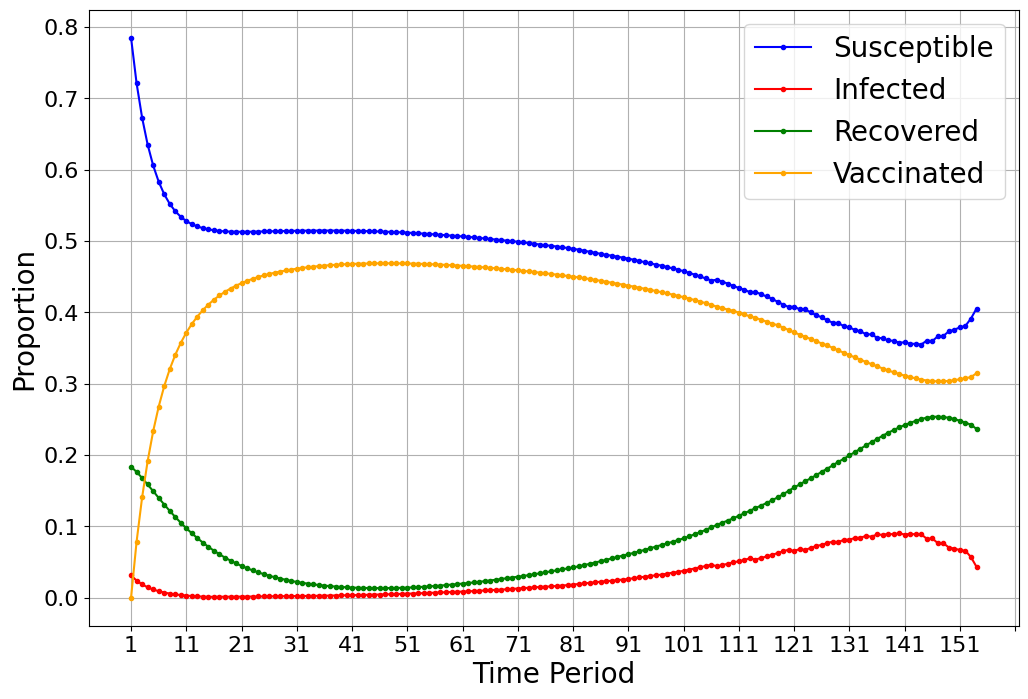
\includegraphics[width=0.42\linewidth]{pics/cumulSIRVDynamicsVax0.1.png}
    %\includegraphics[width=0.48\linewidth]{pics/}
    \caption{Cumulative SIRV and SIR Dynamics in Florida}\label{fig:sir(v)Dynamics}
\end{figure}

\subsection{Unmet Demand}
\begin{figure}
    \centering
    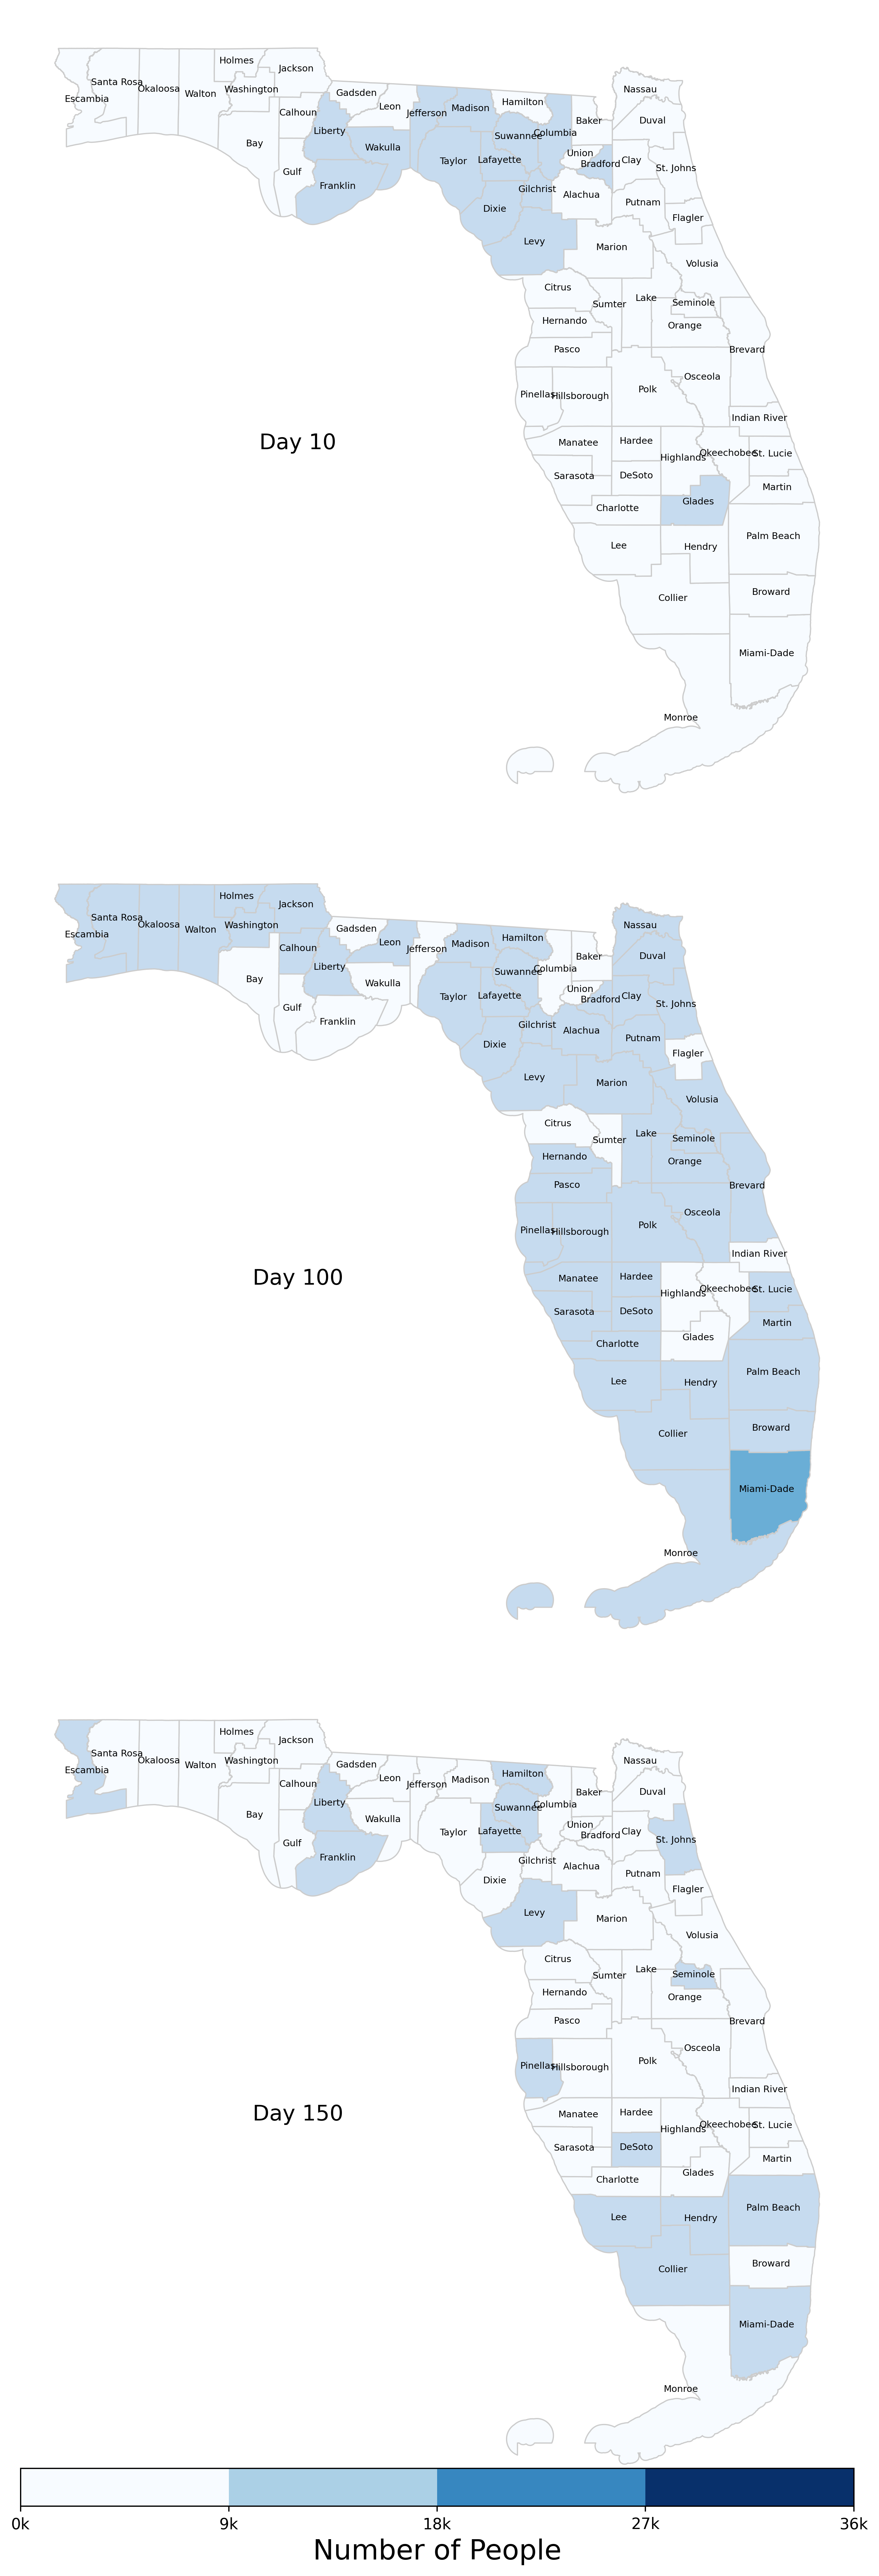
\includegraphics[width=0.43\linewidth]{pics/paperStackedHeatmapVax0.1.png}
    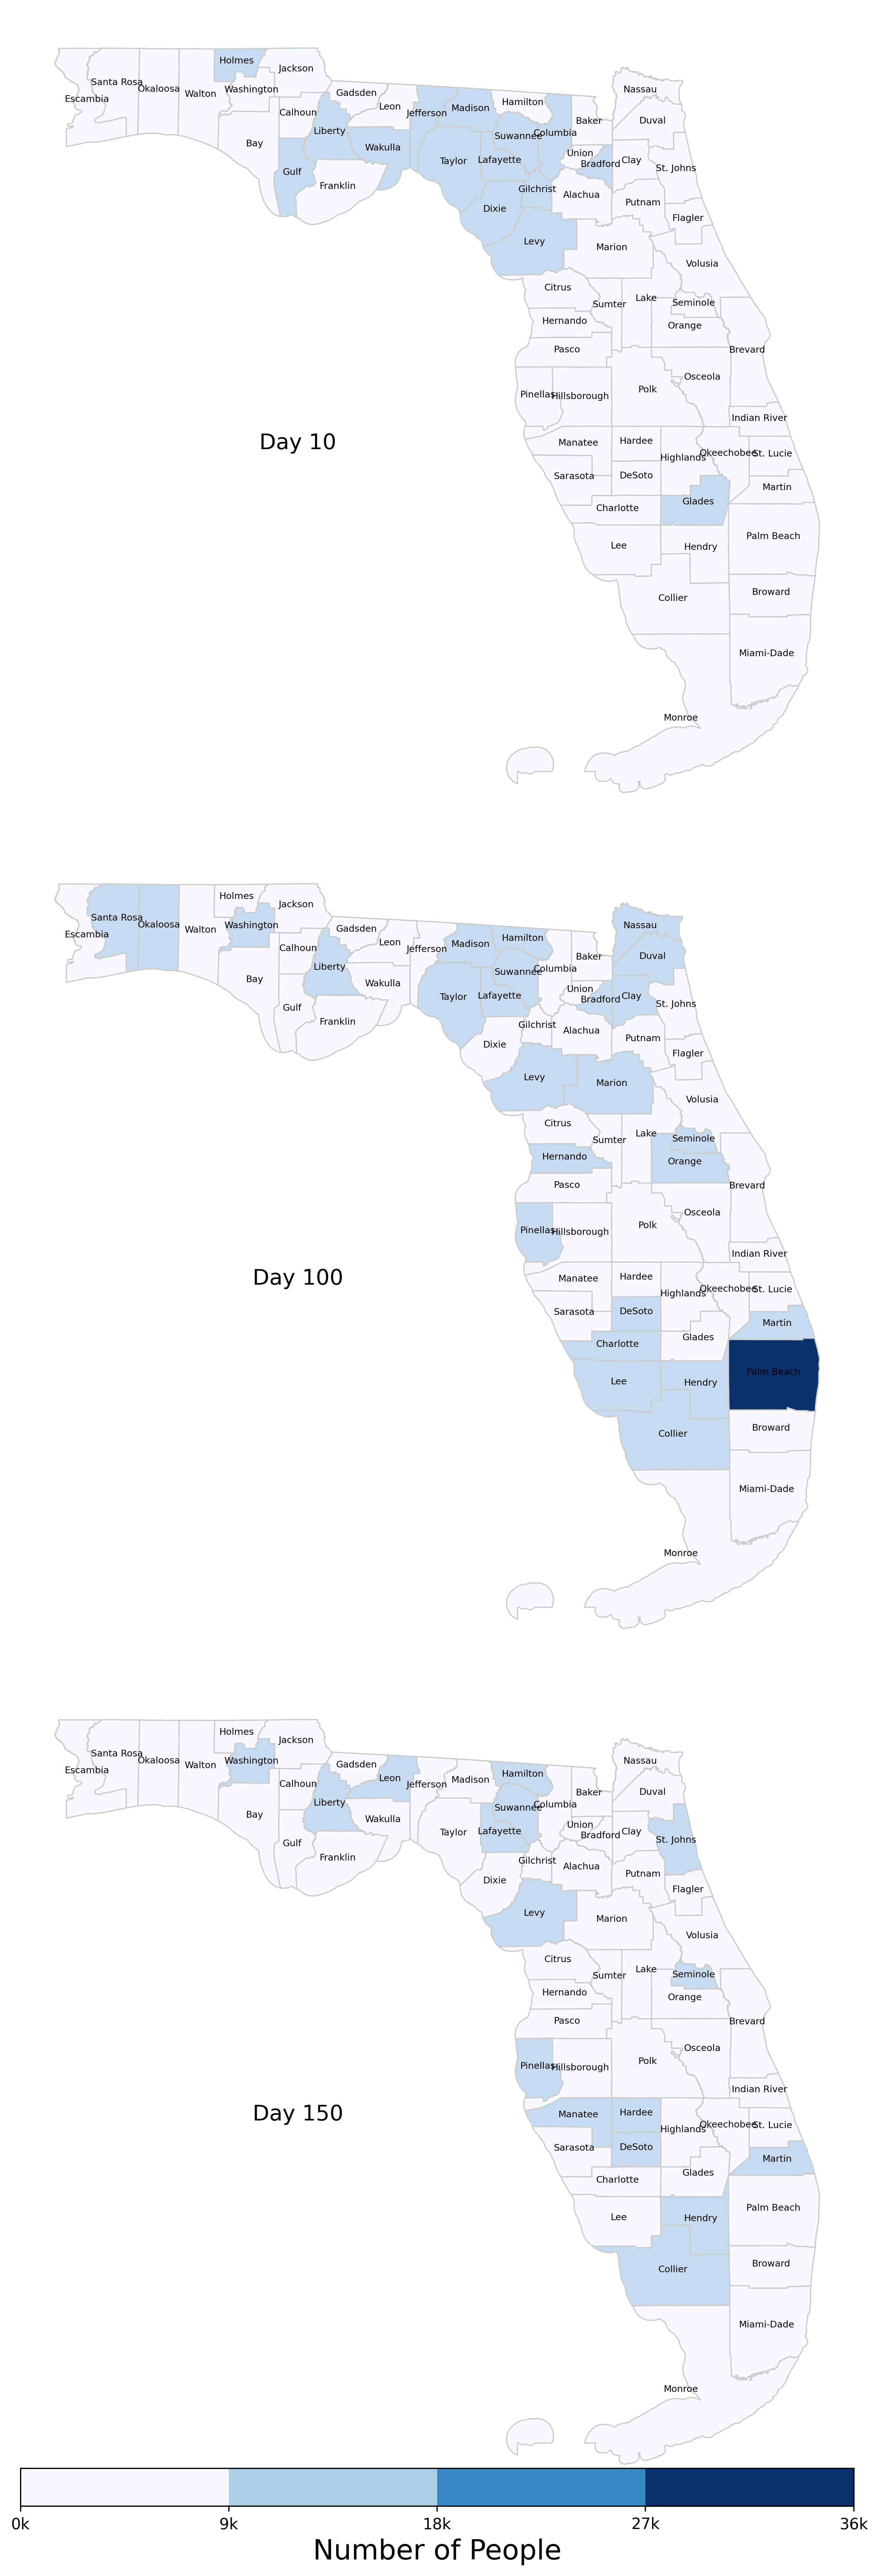
\includegraphics[width=0.43\linewidth]{pics/paperStackedHeatmapNoVax.png}
   \caption{Unmet Demand Heatmap for Vaccinated Scenario (Left) vs. Unvaccinated Scenario (Right)}\label{fig:udHeatmap}
\end{figure}
%\begin{figure}
%    \centering
%    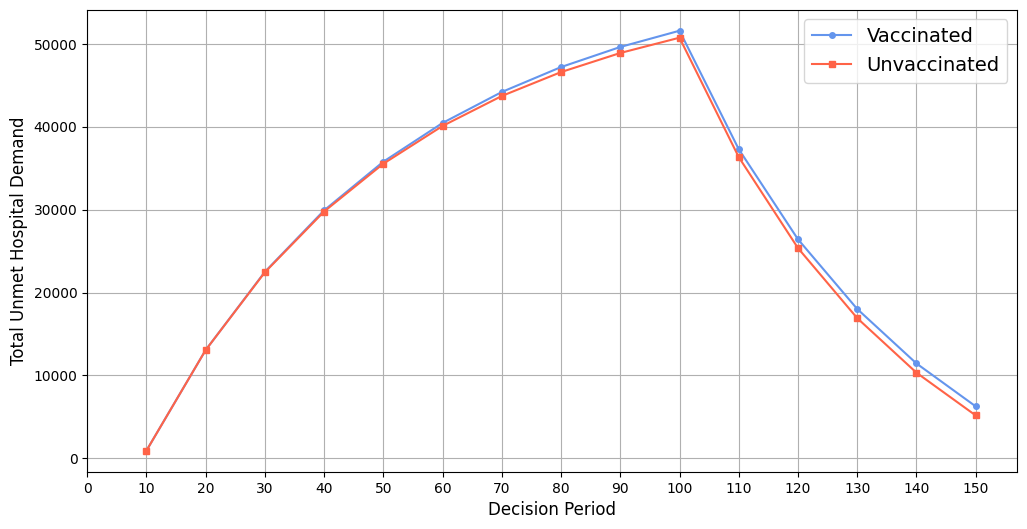
\includegraphics[width=0.42\linewidth]{pics/totalUnmetDemandComparison.png}
%    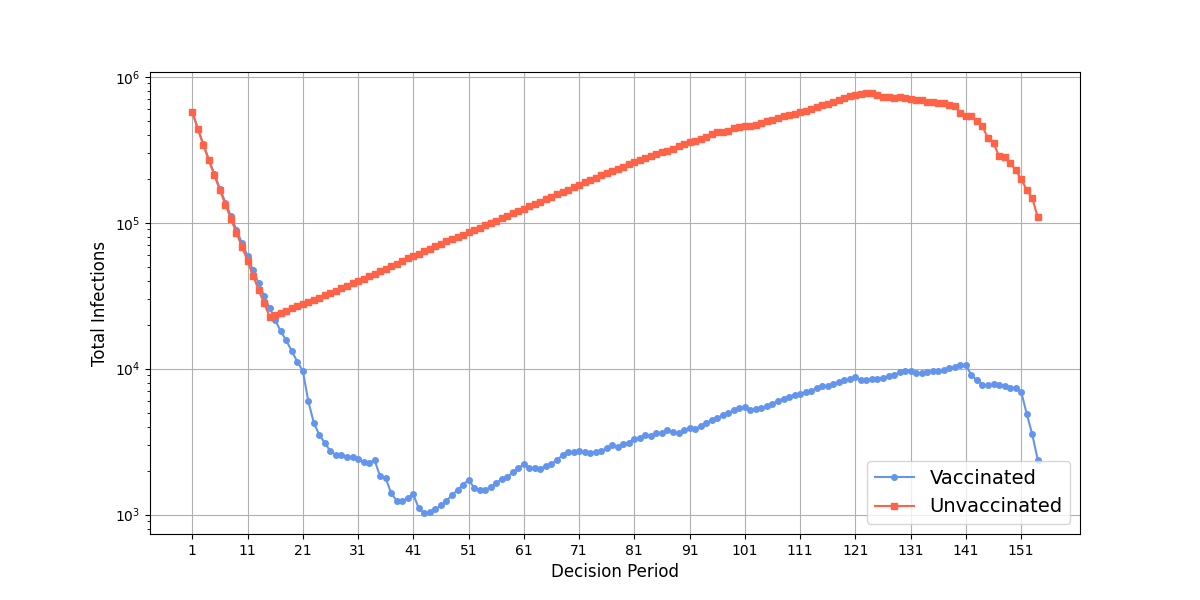
\includegraphics[width=0.48\linewidth]{pics/totalInfectionComparison.png}
%    \caption{Total Unmet Hospital and Demand Infections Across Decision Periods}\label{fig:udInfec}
%\end{figure}

%We observe that unmet hospital demand peaks around day 100, with total infections peaking approximately twenty days later. Figure~\ref{fig:udInfec} demonstrates how, interestingly, unmet hospital demand slightly increases when vaccine dynamics are introduced in the case study, however there are significantly fewer total infections across the time horizon. There are many potential explanations for this phenomenon: 

\subsection{Patient Transfers}
Patient transfers play a critical role in the transmission of infectious diseases, thus they were tracked on all decision periods of our mathematical model. Figure\ref{fig:patientAlloc} displays the patient transfer information for Days 30 and 90 of the model. The thickness of the arrow dictates the volume of the patient transfer, and the direction of the arrow, from tip to tail, demonstrates patients being transferred from county $i$ to county $j$. 

We omit the graphs of the daily in- and out-degrees of each county in Florida patient travel, though we list some of the key insights they reveal. In the vaccinated scenario, large metropolitan counties like Palm Beach, Orange, and Duval counties repeated appear as ``receivers'' of large patient volumes. In general, the large metropolitan areas often sent and received large volumes of patients as they have larger hospital capacities, though a larger number of infections. Other more rural counties, like those in the Panhandle, regularly export patients to nearby regions since they tend to have limited healthcare capacity relative to their infection surges, making them consistent ``senders''. We also observe that with the waning of vaccine effectiveness and immunity observed in Figure\ref{fig:sir(v)Dynamics}, patient transfer drastically increases to account for the surge in infections. Finally, patient transfers occurred consistently throughout the time horizon, indicating that despite vaccination efforts, hospital capacity constraints remained a persistent challenge, necessitating ongoing redistribution of patients to balance demand across regions. 

A common phenomenon that results from constraints (\ref{eq:transfer_limit})-(\ref{eq:binary_constraint}) is the ``chaining'' of patients being transferred to subsequent adjacent counties. Patient transfers create cascading effects during decision periods as hospitals reach capacity. When transferred patients fill available beds in receiving counties, remaining patients requiring care must be redirected elsewhere, leading to further transfers. In general, we observe less transferred patients for the vaccinated scenario (953 thousand) than the unvaccinated scenario (1.10 million).

\begin{figure}
    \centering
    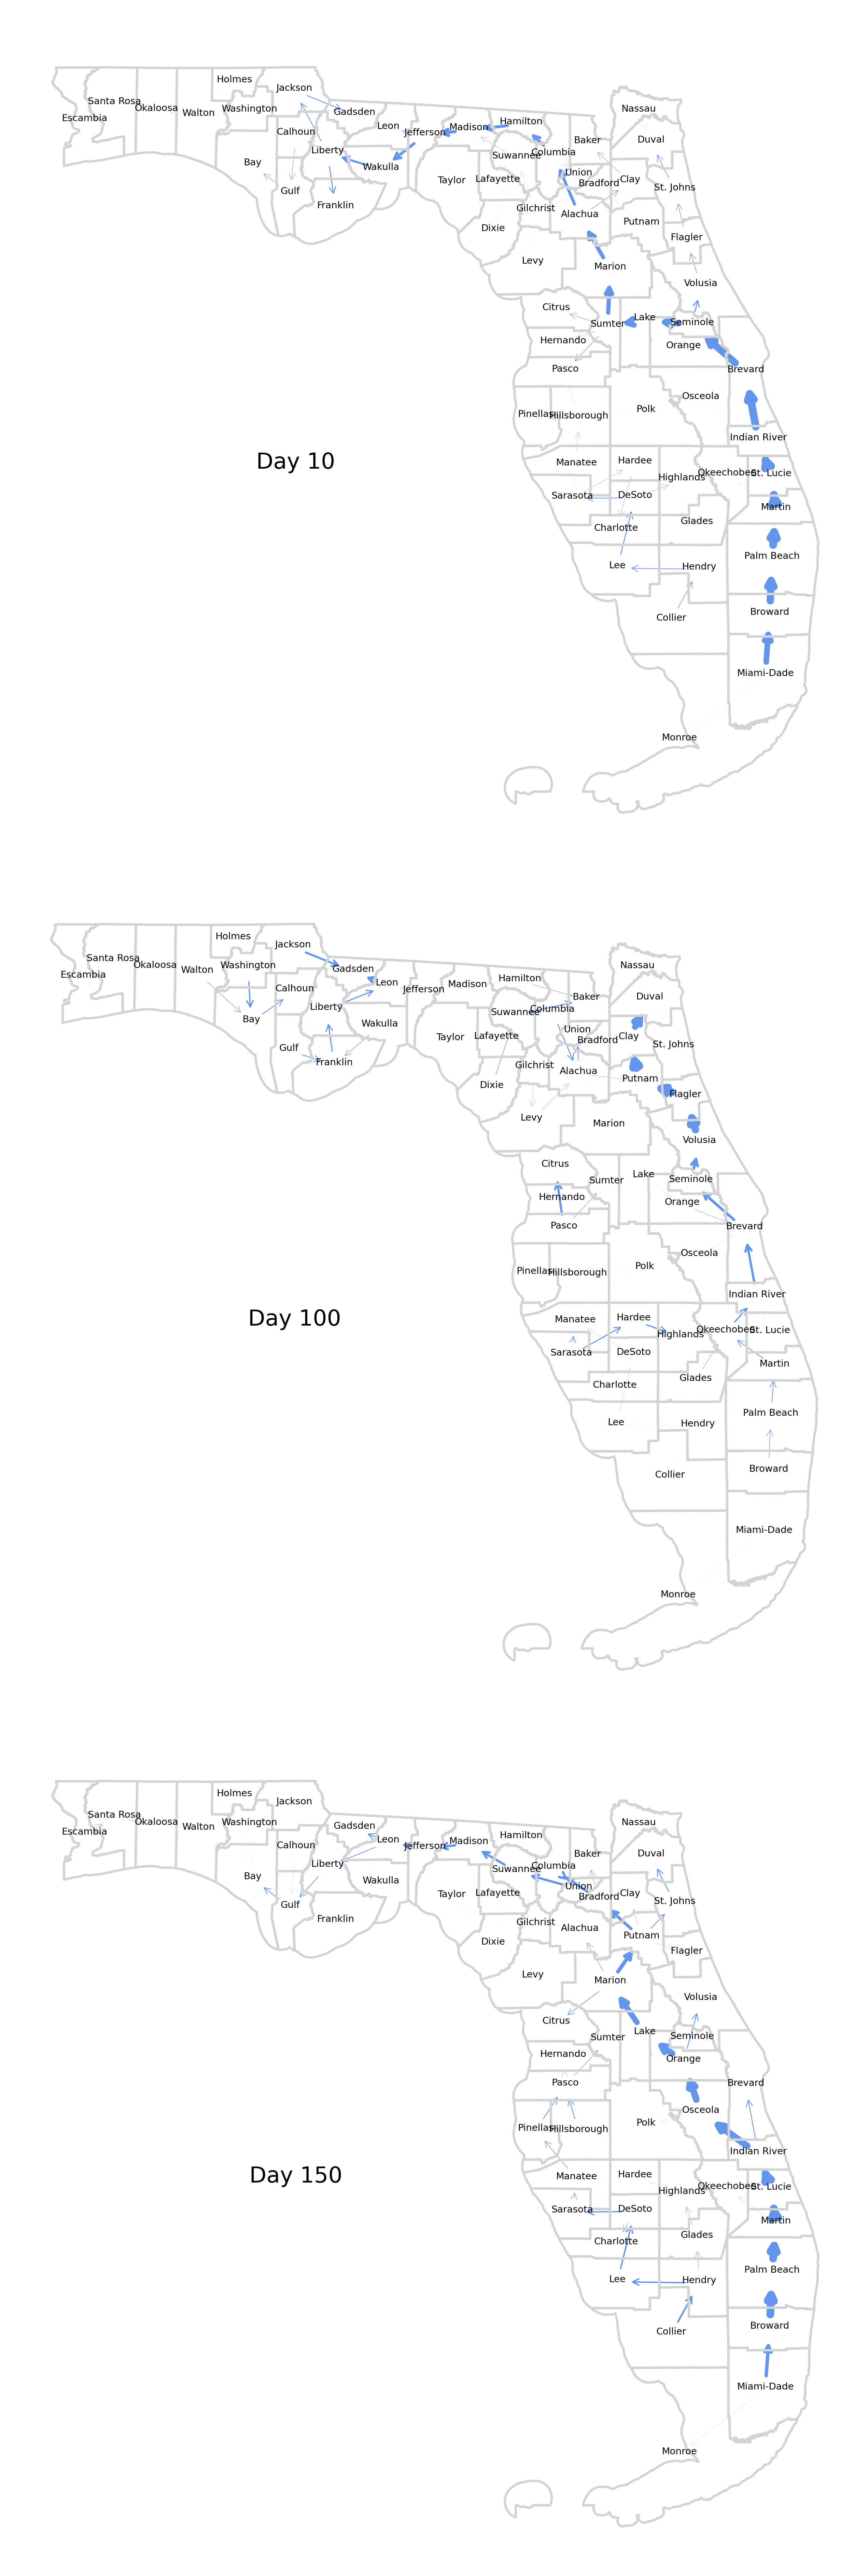
\includegraphics[width=0.43\linewidth]{pics/paperStackedPatientTransfersVax0.1.png}
    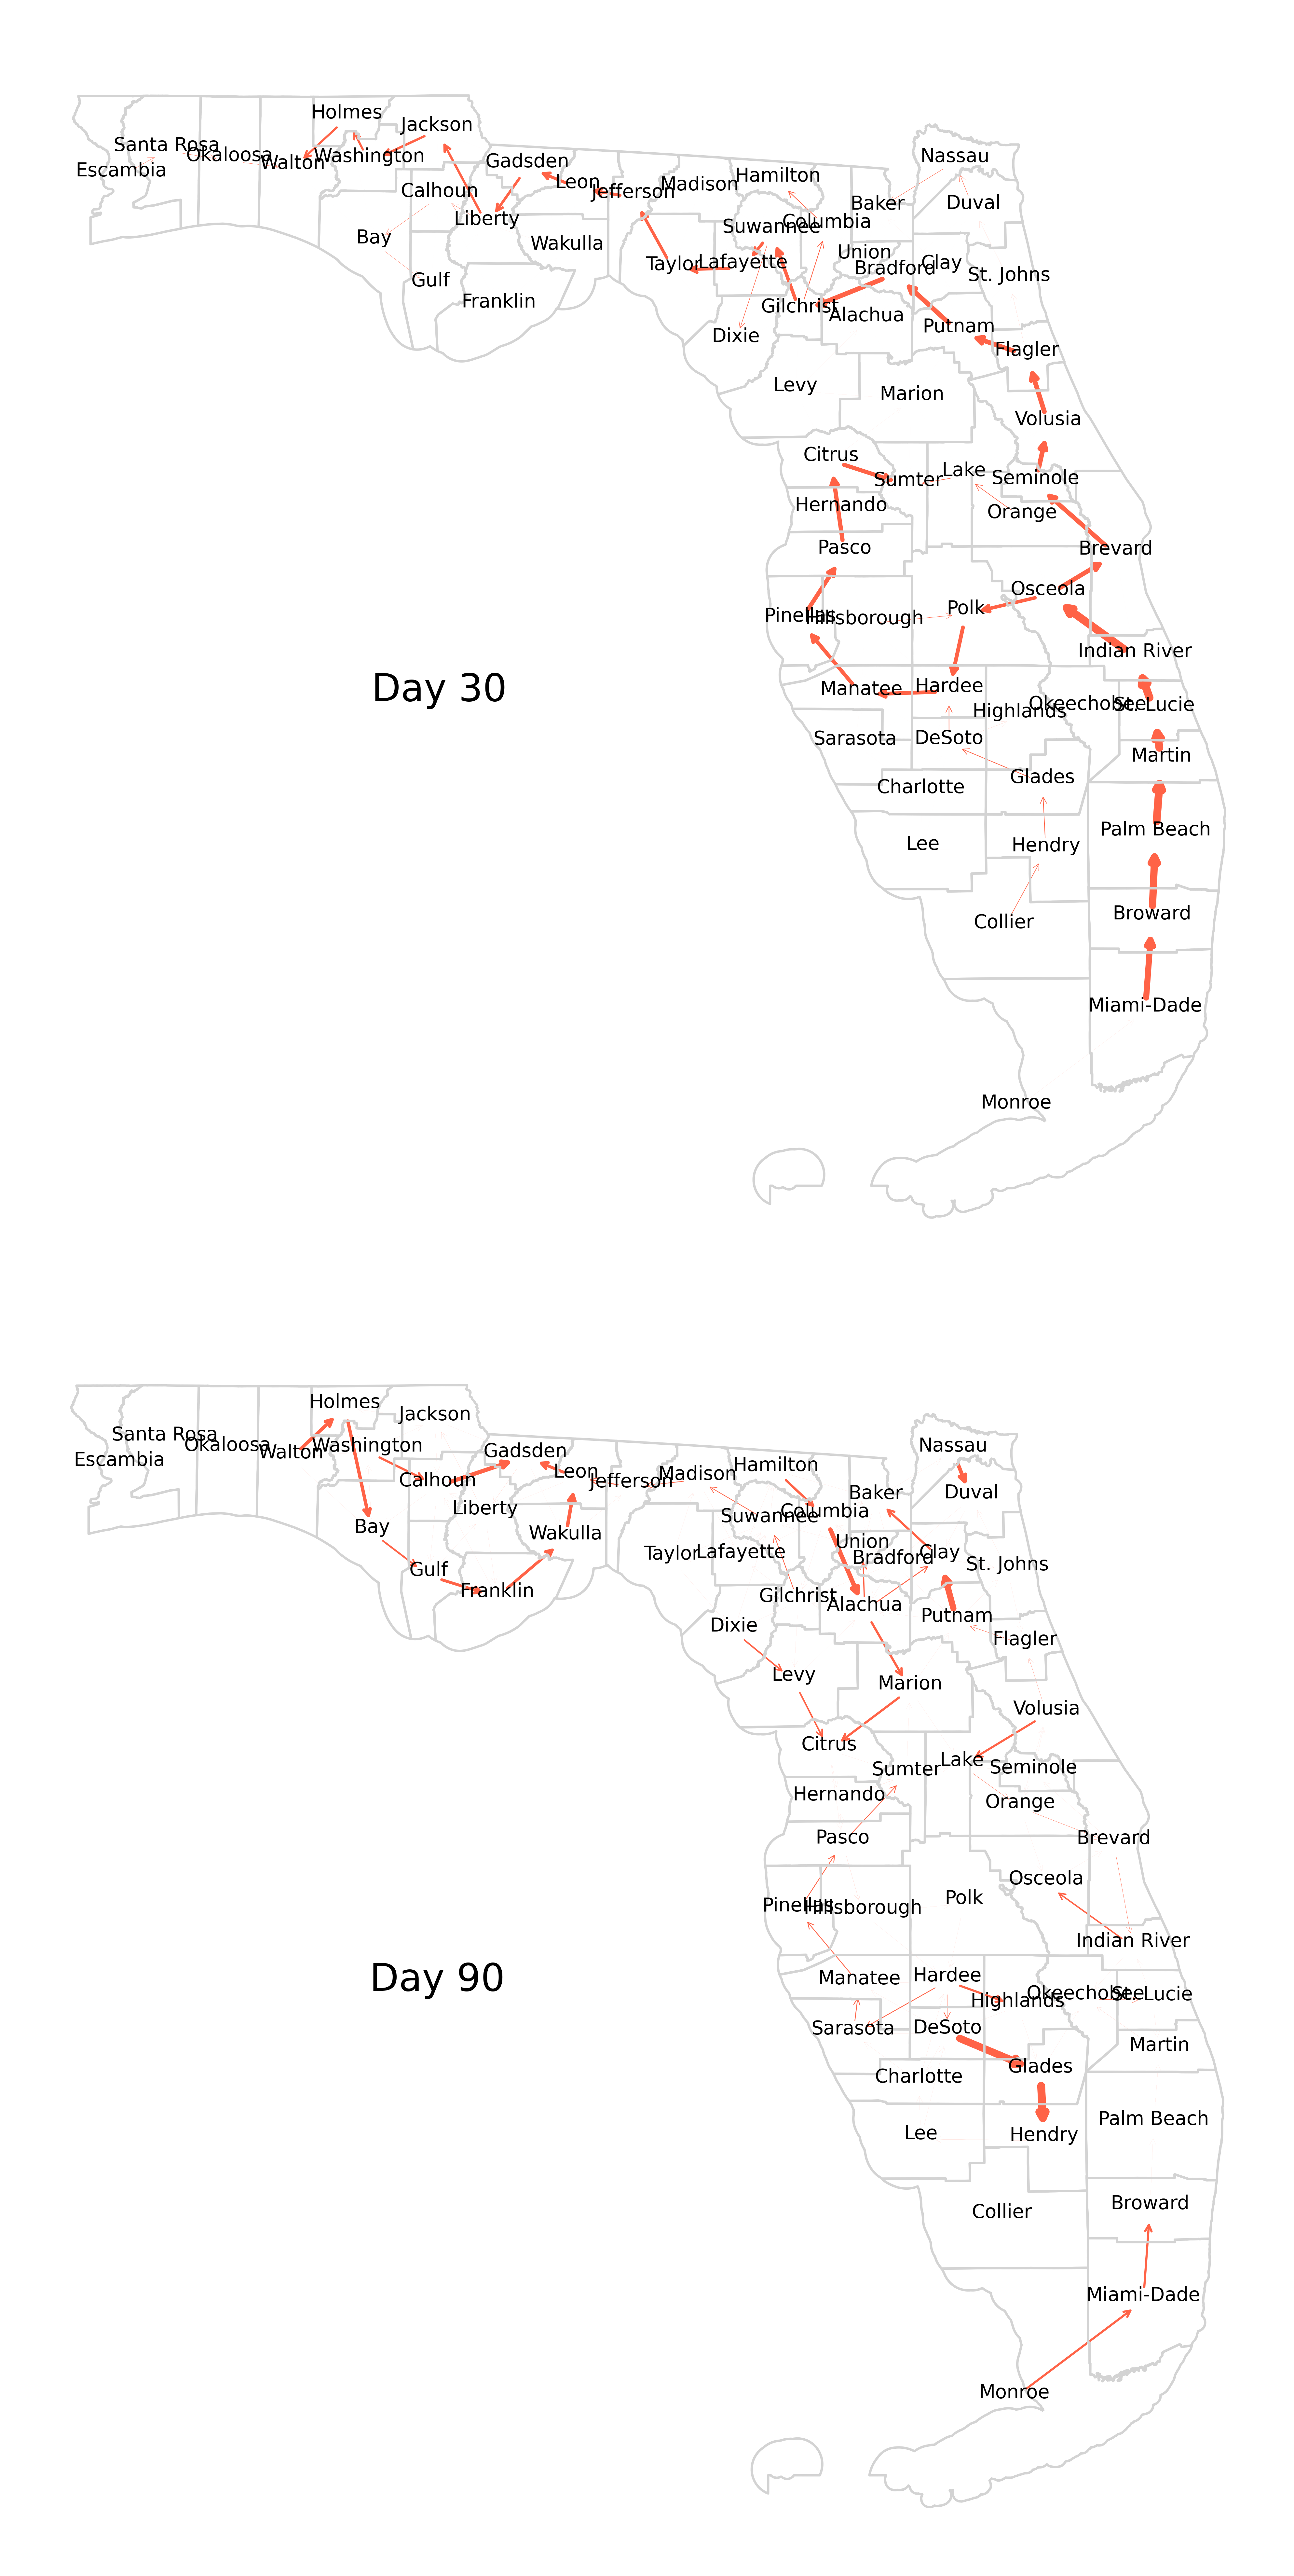
\includegraphics[width=0.43\linewidth]{pics/paperStackedPatientTransfersNoVax.png}
    \caption{Patient Allocation for Vaccinated Scenario (Left) vs. Unvaccinated Scenario (Right)}\label{fig:patientAlloc}
\end{figure}

\section{Conclusions and Future Work}
% fix patient chaining issue. 
% 
\printbibliography[heading=subbibintoc, title={References}]


%\begin{ieombiography}
%  \textbf{Alexander DeLise} is a ...
%  (Limit to 250 words.)
%
%  \noindent \textbf{Seyedreza Abazari} is a....
%
%  \noindent \textbf{Dr. Arda Vanli} is a %professor of ...
%\end{ieombiography}

\end{document}
